\documentclass[conference]{IEEEtran}
%\usepackage{spconf,amsmath,amssymb,graphicx}
\usepackage{amsmath,amssymb,graphicx,caption,listings,hyperref,graphicx}

% Example definitions.
% --------------------
% nice symbols for real and complex numbers
\newcommand{\R}[0]{\mathbb{R}}
\newcommand{\C}[0]{\mathbb{C}}
% bold paragraph titles
\newcommand{\mypar}[1]{{\bf #1.}}
\newcommand{\mysubpar}[2]{{\bf #1.}}
\graphicspath{ {./images/} }

\lstset{frame=tb,
  language=C,
  aboveskip=5mm,
  belowskip=5mm,
  showstringspaces=true,
  columns=flexible,
  numbers=none,	
  breaklines=true,
  breakatwhitespace=true,
  tabsize=2
}

\begin{document}

\title{A Stencil computation algorithm optimization}


\author{\IEEEauthorblockN{Ivan Buccella}
\IEEEauthorblockA{Department of Computer Science\\
 University of Salerno\\
 Italy}
}

\maketitle

\begin{abstract}
This article tries to apply several types of optimizations to a Stencil computation algorithm, in order to minimize the computation execution time. In this document are treated the concepts of OpenMP multithreading code optimizations, loop interchange optimization, parallel loops optimizations, and loop tiling optimizations. From the experiment results, the best optimization to apply to the chosen Stencil computation algorithm is loop tiling. It also tries to increase the algorithm dimension on the optimized code in order to compare the performances increase/decrease.
\end{abstract}

\section{Introduction}\label{sec:intro}

Stencil computation has been a research topic for decades in a variety of domains including computational electromagnetics \cite{taflove}, solution of PDEs using finite difference or finite volume discretizations \cite{smith}, and image processing for CT and MRI imaging \cite{cong-huang-zou}\cite{cong-zou}. In the finite-difference computation process, Stencil computation is often iteratively used to solve the differential operator. In these scientific and engineering applications, Stencil is often the most vital and time-consuming computing kernel \cite{su-zhang-mei}.

The general computation pattern of Stencil computation is that the central point accumulates the contributions of neighbor points in every axis of the Cartesian coordinate system \cite{su-zhang-mei}. The number of neighbor points in each axis or grid step of the Stencil computation corresponds to the accuracy of the Stencil. The more neighbor elements involved in the computation, the higher accuracy the computation obtains. The computation is then repeated for every point of the grid domain as an iterative operator of the PDEs. Due to the structure of the Stencil computation, two inherent problems exist:
\begin{itemize}
	\item First, it is the non-continuous memory access pattern. There exist distances among elements needed for the computation except those in the innermost or unit-stride dimension. Many more cycles in latencies are required to access these points. 
	\item Second, it is the low arithmetic intensity and poor data reuse. Just one point is updated with all the elements loaded. The data reuse between two updates is also limited within the unit-stride dimension, while the other dimensions' elements that are expensive to access have no data reuse at all.
\end{itemize}


\mypar{Motivation} 
On the Stencil computation various optimization approaches have been discussed. The main contributions for Stencil optimization can be divided into two aspects: blocking and parallelism optimizations \cite{su-zhang-mei}.

Blocking optimizations aim at improving the data locality of both space and time dimensions. They are highly related to the tiling strategies widely employed in the modern multi-level cache hierarchy architectures.
 
Parallelism optimizations refer to the techniques that explore parallelism at diverse levels, including data-level parallelisms, such as SIMD, thread-level parallelism, such as block decomposition, and instruction-level parallelism. They tend to make full use of the potential advantages of modern processors' many- or multi-core architectures. 

However, these optimizations can be categorized according to their complexity of implementation (programmer efforts), benefit improvement (performance) and implementation tightness regarding hardware (dependence) \cite{cruz}.

\mypar{Related work} 
In the article `\textit{Acceleration of real-life stencil codes on GPUs}' \cite{barigou} there is a detailed description of the loop tiling transformation, the CUDA programming model, and GPU architecture consists. Then, it explores the possible tiling approaches that can be applied to such Stencil patterns; it describes 3 interesting approaches: 2D tiles, time-skewing+time-tiling transformation, and performing redundant computations inside tiles.

The article `\textit{High-Performance Code Generation for Stencil Computations on GPU Architectures}' \cite{holewinski-pouchet-sadayappan} introduces an automatic code generation scheme for Stencil computations on GPU architectures. This scheme uses overlapped tiling to provide efficient time tiling on GPU architectures, which are massively threaded but are susceptible to performance degradation due to branch divergence and a lack of memory coalescing. 

However, this article tries to apply multi-core architecture optimizations using OpenMP instead of using CUDA programming models and GPU architecture like in the related works.

\section{Background}\label{sec:background}

In order to understand the described work, it is important to know something about multi-core, and code optimizations using OpenMP.

\mypar{The multi-core architecture}
Multicore refers to an architecture in which a single physical processor incorporates the core logic of more than one processor. A single integrated circuit is used to package or hold these processors. These single integrated circuits are known as a die. Multicore architecture places multiple processor cores and bundles them as a single physical processor. The objective is to create a system that can complete more tasks at the same time, thereby gaining better overall system performance \cite{techopedia}.

\mypar{OpenMP}
The OpenMP API supports multi-platform shared-memory parallel programming in C/C++ and Fortran. The OpenMP API defines a portable, scalable model with a simple and flexible interface for developing parallel applications on platforms from the desktop to the supercomputer \cite{openmp}.

\mypar{Loop interchange}
In compiler theory, loop interchange is the process of exchanging the order of two iteration variables used by a nested loop. The variable used in the inner loop switches to the outer loop, and vice versa. It is often done to ensure that the elements of a multi-dimensional array are accessed in the order in which they are present in memory, improving the locality of reference \cite{loop-interchange}.

\mypar{Optimization flags}
Without any optimization option, the compiler's goal is to reduce the cost of compilation and to make debugging produce the expected results. Statements are independent: if you stop the program with a breakpoint between statements, you can then assign a new value to any variable or change the program counter to any other statement in the function and get exactly the results you expect from the source code. 
Turning on optimization flags makes the compiler attempt to improve the performance and/or code size at the expense of compilation time and possibly the ability to debug the program. 
The compiler performs optimization based on the knowledge it has of the program. 
Depending on the target and how the compiler was configured, a slightly different set of optimizations may be enabled at each -O level (\textit{-O0},\textit{-O1},\textit{-O2},\textit{-O3}) \cite{optimization-flags}.

\mypar{Parallel loops}
A parallel for loop is a for loop in which the statements in the loop can be run in parallel: on separate cores, processors, or threads. 
In OpenMP the \textit{parallel loop} construct is a shortcut for specifying a parallel construct containing a loop construct with one or more associated loops and no other statements \cite{omp-parallel}. 

\mypar{Loop tiling}
Loop tiling transformation (or simply tiling) consists of partitioning an iteration domain into many regular and uniform tiles \cite{barigou}. A tile is thus a subset of iteration points. Executing a tile corresponds to the execution of all the iteration points it contains. A tiles execution is atomic, which means if a tile execution starts, it cannot be interrupted until it reaches its last iteration point. This condition implies that no data can be exchanged between two concurrent tiles. This transformation allows data to be accessed in blocks (tiles), with the block size defined as a parameter of this transformation. Each loop is transformed into two loops: one iterating inside each block (intratile) and the other one iterating over the blocks (intertile) \cite{loop-tiling}. 

\section{The applied method}\label{sec:yourmethod}

The main goal of this experiment is to minimize as soon as possible the computation time of the chosen algorithm for Stencil Computation. This operation is done by using the above explained techniques: \textit{loop interchange}, \textit{optimization flags}, \textit{parallel loops} and \textit{loop tiling}.

\mypar{Starting Alogrithm}
First of all, it's important to show what is the used algorithm that the experiment tries to improve.
\begin{lstlisting}
for (x = 1; x < N - 1; x++)
{
		for (y = 1; y < N - 1; y++)
		{
				B[x][y] = a * A[x][y] + b * (A[x - 1][y] + A[x + 1][y] + A[x][y - 1] + A[x][y + 1]);
		}
}
\end{lstlisting}

\mypar{Loop interchange}
The first step is editing the starting algorithm by exchanging the order of the iteration variables \textbf{x} and \textbf{y} used by nested loops. The result is two different algorithms:

\setcounter{lstlisting}{0}
\renewcommand{\lstlistingname}{Algorithm}

\begin{lstlisting}[caption={The starting algorithm},label={lst:loop-interchange-x-y}]
for (x = 1; x < N - 1; x++)
{
		for (y = 1; y < N - 1; y++)
		{
				B[x][y] = a * A[x][y] + b * (A[x - 1][y] + A[x + 1][y] + A[x][y - 1] + A[x][y + 1]);
		}
}
\end{lstlisting}

\begin{lstlisting}[caption={A new algorithm with x and y swapped},label={lst:loop-interchange-y-x}]
for (y = 1; y < N - 1; y++)
{
		for (x = 1; x < N - 1; x++)
		{
				B[x][y] = a * A[x][y] + b * (A[x - 1][y] + A[x + 1][y] + A[x][y - 1] + A[x][y + 1]);
		}
}
\end{lstlisting}

\mypar{Optimization flags}
The next step is editing the optimization flag used for compiling the source code; the clang compiler offers four different flag specifications: O0, O1, O2, and O3. The result is four different commands:

\setcounter{lstlisting}{0}
\renewcommand{\lstlistingname}{Command}

\begin{lstlisting}[caption={Flag -O0},label={lst:optimization-flags-0}]
clang code.c -o code.out -fopenmp -O0
\end{lstlisting}

\begin{lstlisting}[caption={Flag -O1},label={lst:optimization-flags-1}]
clang code.c -o code.out -fopenmp -O1
\end{lstlisting}

\begin{lstlisting}[caption={Flag -O2},label={lst:optimization-flags-2}]
clang code.c -o code.out -fopenmp -O2
\end{lstlisting}

\begin{lstlisting}[caption={Flag -O3},label={lst:optimization-flags-3}]
clang code.c -o code.out -fopenmp -O3
\end{lstlisting}

\mypar{Parallel Loops}
The next step is editing the code by applying the parallel loops optimization. In order to distribute the execution of a loop into multiple threads, it has been used the ``#pragma omp parallel for'' \cite{omp-parallel}\cite{omp-for} directive; this directive opens a parallel region and schedules the loop into multiple threads. The directive could be applied to each loop, also on both. For applying the directive on both loops, it has been used the ``#pragma omp parallel for collapse(2)'' \cite{omp-collapse} directive which is able to distribute two nested loops on multiple threads. The result of this step is three different algorithms:

\setcounter{lstlisting}{2}
\renewcommand{\lstlistingname}{Algorithm}

\begin{lstlisting}[caption={Parallel loop on X},label={lst:parallel-loop-x}]
#pragma omp parallel for
for (x = 1; x < N - 1; x++)
{
		for (y = 1; y < N - 1; y++)
		{
				B[x][y] = a * A[x][y] + b * (A[x - 1][y] + A[x + 1][y] + A[x][y - 1] + A[x][y + 1]);
		}
}
\end{lstlisting}

\begin{lstlisting}[caption={Parallel loop on Y},label={lst:parallel-loop-y}]
for (x = 1; x < N - 1; x++)
{
		#pragma omp parallel for
		for (y = 1; y < N - 1; y++)
		{
				B[x][y] = a * A[x][y] + b * (A[x - 1][y] + A[x + 1][y] + A[x][y - 1] + A[x][y + 1]);
		}
}
\end{lstlisting}

\begin{lstlisting}[caption={Parallel loop on X and Y},label={lst:parallel-loop-x-y}]
#pragma omp parallel for collapse(2)
for (x = 1; x < N - 1; x++)
{
		for (y = 1; y < N - 1; y++)
		{
				B[x][y] = a * A[x][y] + b * (A[x - 1][y] + A[x + 1][y] + A[x][y - 1] + A[x][y + 1]);
		}
}
\end{lstlisting}

\mypar{Loop tiling}
The next step is editing the code by applying tiling optimization. In order to apply this type of optimization it has been necessary to cut the \textbf{A} matrix into multiple smaller \textit{tiles}; due to it has been introduced into the code a new variable ``tile\textunderscore size'' which expresses the tile size, and two nested loops that have the goal of executing the code on the different tiles. On the tiling loops (with \textit{xx} and \textit{yy} variables) it has been applied the ``#pragma omp parallel for collapse(2)'' directive in order to distribute the matrices tiles on multiple threads. Different tile sizes have been chosen depending on several points of view like L2 Cache size, etc. The result of this step is four different algorithms, identical but with different tile sizes:

\renewcommand{\lstlistingname}{Algorithm}

\begin{lstlisting}[caption={Loop tiling with size of 16384},label={lst:tiling-1}]
const int tile_size = 16384;
#pragma omp parallel for collapse(2)
for (int xx = 0; xx < N; xx += tile_size)
{
		for (int yy = 0; yy < N; yy += tile_size)
		{
				for (x = xx + 1; x < MIN(xx + tile_size, N - 1); x++)
				{
						for (y = yy + 1; y < MIN(yy + tile_size, N - 1); y++)
						{
								B[x][y] = a * A[x][y] + b * (A[x - 1][y] + A[x + 1][y] + A[x][y - 1] + A[x][y + 1]);
						}
				}
		}
}
\end{lstlisting}

\begin{lstlisting}[caption={Loop tiling with size of 10922},label={lst:tiling-2}]
const int tile_size = 10922;
...same as before
\end{lstlisting}

\begin{lstlisting}[caption={Loop tiling with size of 8192},label={lst:tiling-3}]
const int tile_size = 8192;
...same as before
\end{lstlisting} 

\begin{lstlisting}[caption={Loop tiling with size of 5461},label={lst:tiling-4}]
const int tile_size = 5461;
...same as before
\end{lstlisting}

\mypar{Dimension augmentation}
The next step is editing the \textit{tiled} code by applying two more dimensions to the original Stencil code. In order to apply this step, it has been necessary to edit the internal loops (with \textit{x} and \textit{y} variables) condition from ``MIN(xx + tile\textunderscore size, N - 1)'' to ``MIN(xx + tile\textunderscore size, N - 3)''. Because of the tiling optimization, the code has been executed on different tile sizes depending on several points of view like L2 Cache size, etc. The result of this step is four different algorithms, identical but with different tile sizes:

\renewcommand{\lstlistingname}{Algorithm}

\begin{lstlisting}[caption={Dimension augmentation + loop tiling with size of 16384},label={lst:augmentation-1}]
const int tile_size = 16384;
#pragma omp parallel for collapse(2)
for (int xx = 0; xx < N; xx += tile_size)
{
		for (int yy = 0; yy < N; yy += tile_size)
		{
				for (x = xx + 3; x < MIN(xx + tile_size, N - 3); x = x + 3)
				{
						for (y = yy + 3; y < MIN(yy + tile_size, N - 3); y = y + 3)
						{
								B[x][y] = a * A[x][y] + b * (A[x - 3][y] + A[x - 2][y] + A[x - 1][y] + A[x + 1][y] + A[x + 2][y] + A[x + 3][y] + A[x][y - 3] + A[x][y - 2] + A[x][y - 1] + A[x][y + 1] + A[x][y + 2] + A[x][y + 3]);
						}
				}
		}
}
\end{lstlisting}

\begin{lstlisting}[caption={Dimension augmentation + loop tiling with size of 10922},label={lst:augmentation-2}]
const int tile_size = 10922;
...same as before
\end{lstlisting}

\begin{lstlisting}[caption={Dimension augmentation + loop tiling with size of 8192},label={lst:augmentation-3}]
const int tile_size = 8192;
...same as before
\end{lstlisting} 

\begin{lstlisting}[caption={Dimension augmentation + loop tiling with size of 5461},label={lst:augmentation-4}]
const int tile_size = 5461;
...same as before
\end{lstlisting}

\section{Experimental Results}\label{sec:exp}

\mypar{Experimental setup} The execution timing is obtained by using the OpenMP primitives \cite{omp-get-wtime}, an example is shown in Algorithm \ref{lst:omp-get-time-alg}. The OpenMP settings are shown in Algorithm \ref{lst:omp-configs-alg}. The experiment is executed on two matrices, A and B (initialized with the Algorithm \ref{lst:initialization-alg}), with a size of constant \textbf{N = 32768} and on a PC with current specifications: 
\begin{itemize}
	\item \textbf{CPU}
	\begin{itemize}
		\item \textbf{Model name}: Intel(R) Core(TM) i5-9600K CPU @ 3.70GHz
		\item \textbf{CPU(s)}: 6
		\item \textbf{Socket(s)}: 1
		\item \textbf{Core(s) per socket}: 6
		\item \textbf{Thread(s) per core}: 1
		\item \textbf{Cache L1d}: 192 KiB (6 instances)
		\item \textbf{Cache L1i}: 192 KiB (6 instances)
		\item \textbf{Cache L2}: 1.5 MiB (6 instances)
		\item \textbf{Cache L3}: 9 MiB (1 instance)
		\item \textbf{Intel Hyper-Threading Technology}: No
	\end{itemize}
	\item \textbf{Memory} 
	\begin{itemize}
		\item \textbf{Size}: 26164116 kB
	\end{itemize}
	\item \textbf{Compiler}: clang 14.0.5 with OpenMP 5.0
	\end{itemize}
\end{itemize}

\renewcommand{\lstlistingname}{Algorithm}

\begin{lstlisting}[caption={An example of code for obtaining the execution timing},label={lst:omp-get-time-alg}]
double t_init = omp_get_wtime()
//Your code's here
printf("\%0.15f", omp_get_wtime() - t_init);
\end{lstlisting}

\begin{lstlisting}[caption={OpenMP Configs},label={lst:omp-configs-alg}]
int n_threads = omp_get_max_threads();
omp_set_max_active_levels(1);
omp_set_num_threads(n_threads);
omp_set_dynamic(0);
\end{lstlisting}

\begin{lstlisting}[caption={A and B matrices initialization},label={lst:initialization-alg}]
float **A = (float **)malloc(N * sizeof(float *));
float **B = (float **)malloc(N * sizeof(float *));
for (x = 0; x < N; x++)
{
		A[x] = (float *)malloc(N * sizeof(float));
		B[x] = (float *)malloc(N * sizeof(float));
		for (y = 0; y < N; y++)
		{
				A[x][y] = 1.0f;
				B[x][y] = 0.0f;
		}
}
\end{lstlisting}

\mypar{Results}
Here the following are represented the execution timings for every experiment that has been done.

\begin{itemize}
	\item \textbf{Loop interchange} computation time of: 
	\begin{itemize}
		\item the Algorithm \ref{lst:loop-interchange-x-y} is: 5.0533 (s) 
		\item the Algorithm \ref{lst:loop-interchange-y-x} is: 55.8343 (s)
	\end{itemize}
	\begin{figure}[htbp]
		\centering
			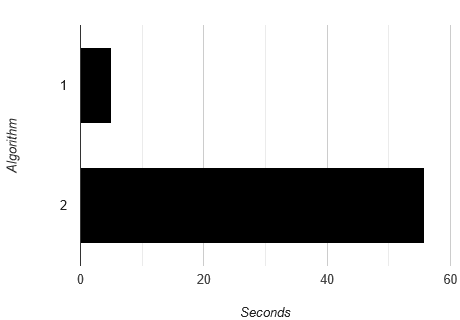
\includegraphics[width=0.50\textwidth]{loop-interchange.png}
		\caption{Loop interchange computation timings}
		\label{fig:loop-interchange}
	\end{figure}
	\item \textbf{Optimization flags}:
	\begin{itemize}
		\item the Algorithm \ref{lst:loop-interchange-x-y} by compiling with the command \ref{lst:optimization-flags-0} is: 5.0493 (s)
		\item the Algorithm \ref{lst:loop-interchange-x-y} by compiling with the command \ref{lst:optimization-flags-1} is: 1.3734 (s)
		\item the Algorithm \ref{lst:loop-interchange-x-y} by compiling with the command \ref{lst:optimization-flags-2} is: 0.5931 (s)
		\item the Algorithm \ref{lst:loop-interchange-x-y} by compiling with the command \ref{lst:optimization-flags-3} is: 0.5904 (s)
	\end{itemize}
	\begin{figure}[htbp]
		\centering
			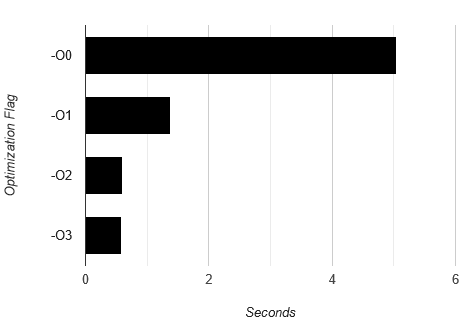
\includegraphics[width=0.50\textwidth]{optimization-flags.png}
		\caption{Optimization flags computation timings}
		\label{fig:optimization-flags}
	\end{figure}	
	\item \textbf{Parallel loops}: 
	\begin{itemize}
		\item the Algorithm \ref{lst:parallel-loop-x} is: 0.4585 (s)
		\item the Algorithm \ref{lst:parallel-loop-y} is: 0.4760 (s)
		\item the Algorithm \ref{lst:parallel-loop-x-y} is: 0.7419 (s)
	\end{itemize}
	\begin{figure}[htbp]
		\centering
			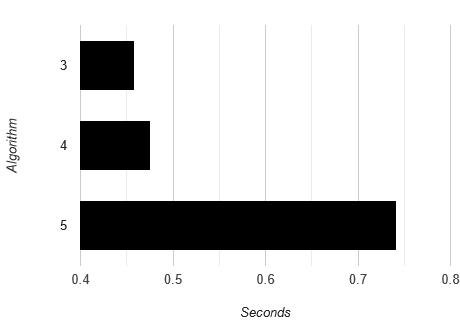
\includegraphics[width=0.50\textwidth]{parallel-loops.png}
		\caption{Parallel loops computation timings}
		\label{fig:parallel-loops}
	\end{figure}		
	\item \textbf{Loop tiling}: 
	\begin{itemize}
		\item the Algorithm \ref{lst:tiling-1} is: 0.4451 (s)
		\item the Algorithm \ref{lst:tiling-2} is: 0.4599 (s)
		\item the Algorithm \ref{lst:tiling-3} is: 0.4422 (s)
		\item the Algorithm \ref{lst:tiling-4} is: 0.4537 (s)
	\end{itemize}	
	\begin{figure}[htbp]
		\centering
			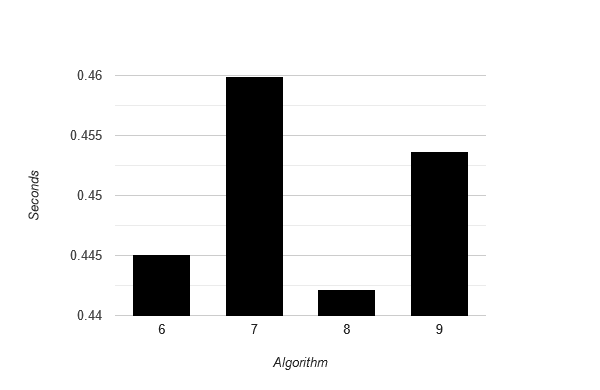
\includegraphics[width=0.50\textwidth]{loop-tiling.png}
		\caption{Loop tiling computation timings}
		\label{fig:loop-tiling}
	\end{figure}		
	\item \textbf{Dimension augmentation}: 
	\begin{itemize}
		\item the Algorithm \ref{lst:augmentation-1} is: 0.2649 (s)
		\item the Algorithm \ref{lst:augmentation-2} is: 0.2911 (s)
		\item the Algorithm \ref{lst:augmentation-3} is: 0.2645 (s)
		\item the Algorithm \ref{lst:augmentation-4} is: 0.2676 (s)
	\end{itemize}	
	\begin{figure}[htbp]
		\centering
			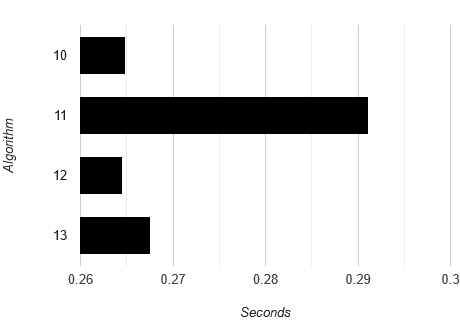
\includegraphics[width=0.50\textwidth]{dimension-augmentation.png}
		\caption{Dimension augmentation computation timings}
		\label{fig:dimension-augmentation}
	\end{figure}
\end{itemize}

\section{Conclusions}
This article presents a number of different approaches to optimize the above-detailed Stencil computations algorithm on multi-core architectures, based on a
range of micro benchmarks.
For the \textbf{loop interchange} optimization, it indicates that the standard loop \textit{x-y} is faster than the \textit{y-x} loop, this is favored by the C programming language memory layout.
For the \textbf{optimization flags} optimization, it indicates that the best flag to use for compiling the code is the -O3.
For the \textbf{parallel loop} optimization, it indicates that having only one parallel loop on the external loop is faster.
For the \textbf{loop tiling} optimization, it indicates that having a \textit{tile\textunderscore size} of \textit{8192} is faster.
About the \textbf{dimension} of the Stencil computation algorithm, it shows that by augmenting the number of dimensions of two, the computation is faster with \textbf{loop tiling} optimization than having a lower number of dimensions.

In future work, would be interesting to try to implement what is the maximum number of dimension augmentation that offers a lower computation timing.


\begin{thebibliography}{1}

\bibitem{taflove}
A. Taflove. Computational electrodynamics: The finite-difference time-domain method. 1995.

\bibitem{smith}
G. Smith. Numerical Solution of Partial Differential Equations: Finite Difference Methods. Oxford University Press, 2004.

\bibitem{cong-huang-zou}
J. Cong, M. Huang, and Y. Zou. Accelerating fluid registration algorithm on multi-FPGA platforms. FPL, 2011.

\bibitem{cong-zou}
On the Transformation Optimization for Stencil Computation

\bibitem{su-zhang-mei}
Huayou Su *, Kaifang Zhang and Songzhu Mei. On the Transformation Optimization for Stencil Computation

\bibitem{cruz}
Cruz, R.D.L.; Araya-Polo, M. Algorithm 942: Semi-Stencil. ACM Trans. Math. Softw. 2014, 40, 1–39.

\bibitem{barigou}
Youcef Barigou. Acceleration of real-life stencil codes on GPUs. Hardware Architecture [cs.AR]. 2011.

\bibitem{holewinski-pouchet-sadayappan}
Justin Holewinski, Louis-Noël Pouchet, P. Sadayappan. High-Performance Code Generation for Stencil Computations on GPU Architectures.

\bibitem{techopedia}
\href{https://www.techopedia.com/definition/5305/multicore}{Multi-core}

\bibitem{openmp}
\href{https://www.openmp.org/}{OpenMP}

\bibitem{loop-interchange}
\href{https://en.wikipedia.org/wiki/Loop_interchange}{Loop interchange}

\bibitem{optimization-flags}
\href{https://gcc.gnu.org/onlinedocs/gcc/Optimize-Options.html}{Options That Control Optimization}
 
\bibitem{loop-tiling}
João M.P.Cardoso, José Gabriel F. Coutinho, Pedro C. Diniz. Chapter 5 - Source code transformations and optimizations. Embedded Computing for High Performance

\bibitem{omp-get-wtime}
\href{https://www.openmp.org/spec-html/5.0/openmpsu160.html}{omp\textunderscore get\textunderscore wtime() function}

\bibitem{omp-parallel} 
\href{https://www.openmp.org/specifications/}{OpenMP API 5 Specification. OMP Parallel.}

\bibitem{omp-for}
\href{https://www.openmp.org/specifications/}{OpenMP API 5 Specification. OMP For.}

\bibitem{omp-collapse}
\href{https://www.openmp.org/specifications/}{OpenMP API 5 Specification. Collapse.}

\end{thebibliography}

\end{document}


